\documentclass[notheorems,serif,table,compress]{beamer}  %dvipdfm选项是关键,否则编译统统通不过
%%------------------------常用宏包------------------------
%%注意, beamer 会默认使用下列宏包: amsthm, graphicx, hyperref, color, xcolor, 等等
\usepackage{fontspec,xunicode,xltxtra}  % for XeTeX
\usepackage{verbatim}
\usepackage{mathabx}
\usepackage{latexsym}
\usepackage{amsfonts,amssymb}
\usepackage{styles/iplouclistings}
\usepackage{fancybox}
\usepackage{colortbl}
\usepackage{tcolorbox}
%\usepackage[T1]{fontenc}
%\usepackage{bookman}
\usepackage{subfigure}
\usepackage{hyperref}
\usepackage{listings}
\usepackage{animate}
\usepackage[absolute,overlay]{textpos}
\usepackage{graphicx}
\usepackage{tikz}
\usepackage[americaninductors,europeanresistors]{circuitikz}
\usepackage{tikz}
\usepackage{fancybox}     %% 定义zhushadow时用到
\newsavebox{\mysaveboxOne}  %%为了在only中使用lstlisting
\newsavebox{\mysaveboxTwo}
\newsavebox{\mysaveboxThree}
\newsavebox{\mysaveboxFour}
\newsavebox{\mysaveboxFive}
\newsavebox{\mysaveboxSix}
\newsavebox{\mysaveboxSeven}
\newcommand\zhushadow[2][purple]{\hskip5pt\shadowbox{\color{#1}\small\kai #2\vspace{3mm}}}

%%------------------------ThemeColorFont------------------------
%% Presentation Themes
% \usetheme[<options>]{<name list>}
%\usetheme{Madrid}
\usetheme{Berkeley}
%% Inner Themes双精度计算
% \useinnertheme[<options>]{<name>}
%% Outer Themes
% \useoutertheme[<options>]{<name>}
%\useoutertheme{miniframes} 
%% Color Themes 
%\usecolortheme[<options>]{<name list>}
%% Font Themes
\usefonttheme{serif}
\setbeamertemplate{background canvas}[vertical shading][bottom=white,top=structure.fg!7] %%背景色, 上25%的蓝, 过渡到下白.
\setbeamertemplate{theorems}[numbered]
\setbeamertemplate{navigation symbols}{}   %% 去掉页面下方默认的导航条.
\usepackage{styles/zhfontcfg}
%\setsansfont[Mapping=tex-text]{文泉驿正黑}  %% 需要fontspec宏包
     %如果装了Adobe Acrobat,可在font.conf中配置Adobe字体的路径以使用其中文字体
     %也可直接使用系统中的中文字体如SimSun,SimHei,微软雅黑 等
     %原来beamer用的字体是sans family;注意Mapping的大小写,不能写错
     %设置字体时也可以直接用字体名,以下三种方式等同:
     %\setromanfont[BoldFont={黑体}]{宋体}
     %\setromanfont[BoldFont={SimHei}]{SimSun}
     %\setromanfont[BoldFont={"[simhei.ttf]"}]{"[simsun.ttc]"}
%%------------------------MISC------------------------
\graphicspath{{figures/}}         %% 图片路径. 本文的图片都放在这个文件夹里了.
%%------------------------listing------------------------
%\lstset{language=[LaTeX]TeX,Python}
%%------------------------正文------------------------
\begin{document}
\XeTeXlinebreaklocale "zh"         % 表示用中文的断行
\XeTeXlinebreakskip = 0pt plus 1pt % 多一点调整的空间
%%----------------------------------------------------------
%% This is only inserted into the PDF information catalog. Can be left
%% out.
%%%
%% Delete this, if you do not want the table of contents to pop up at
%% the beginning of each subsection:
%\AtBeginSection[]{                              % 在每个Section前都会加入的Frame
%  \frame<handout:0>{
%    \frametitle{Contents}\small
%    \tableofcontents[current,currentsubsection]
%  }
%}
%
%\AtBeginSubsection[]                            % 在每个子段落之前
%{
%  \frame<handout:0>                             % handout:0 表示只在手稿中出现
%  {
%    \frametitle{Contents}\small
%    \tableofcontents[current,currentsubsection] % 显示在目录中加亮的当前章节
%  }
%}

\setbeamertemplate{caption}{\raggedright\insertcaption\par}

%%----------------------------------------------------------
\logo{
\includegraphics[scale=0.07]{ouc-logo.jpg}}
\title{Saliency Detection}
%\subtitle{Bottom-Up Saliency Detection Model Based on Human Visual Sensitivity and Amplitude Spectrum}
\author[]{\textcolor{olive}{Zhu Yafei}}
\institute[CVBIOUC]
{
\small\textcolor{violet}{CVBIOUC\\
Ocean University of China\\
\url{http://vision.ouc.edu.cn/~zhenghaiyong}}
}
\date[March 20, 2015]{March 20, 2015}
%\titlegraphic{
%
\includegraphics[height=1.0cm]{ouc-logo.jpg}}
\frame{ \titlepage }
%%----------------------------------------------------------
%\section*{Contents}
\frame{\frametitle{Contents}\tableofcontents}
%%----------------------------------------------------------
\def\hilite<#1>{\temporal<#1>{\color{blue!15}}{\color{black}}{\color{black}}}
\newcommand{\shadow}[2][purple]{\hskip5pt\shadowbox{\color{#1}\small \kai #2\vspace{3mm}}}
\newcommand{\colorrbox}[2][purple]{\doublebox{\color{#1}\small \kai#2}}

%============================================================================

\section{Introduction}

%==========================================================================


%\begin{frame}
%\frametitle{What?}
%
%%\begin{tikzpicture}[remember picture,overlay]
%%             \fill [write] (current page.south west) rectangle (current page.north east);
%%             \node at (current page.center) {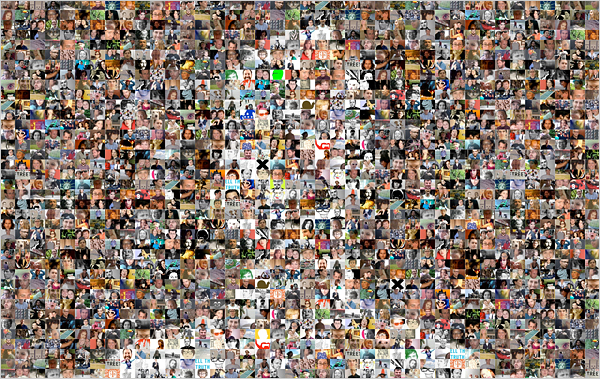
\includegraphics{people}};
%%\end{tikzpicture}
%\begin{textblock*}{8cm}(1.55cm,1.55cm)
%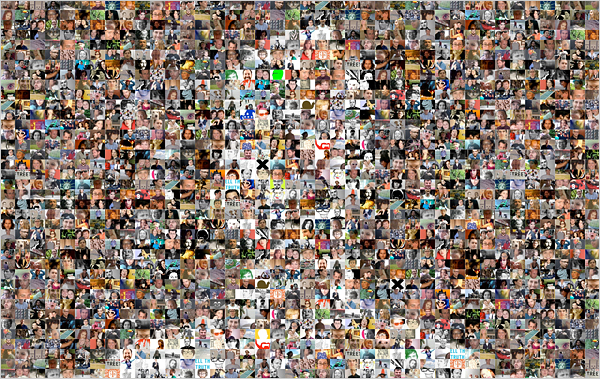
\includegraphics[width=13cm]{people}
%\end{textblock*}
%%\vspace{0in}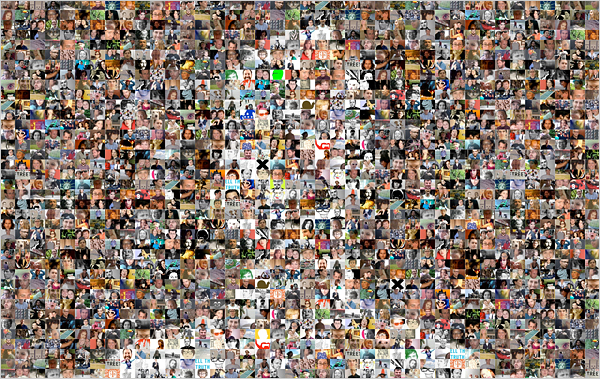
\includegraphics[width=\paperwidth]{people}
%The eyes capture light which results in information in the order of 109 bits every second.
%\end{frame}


\begin{frame}[fragile]
  \frametitle{What?}
  \only<1>{
  A rich stream of visual data ($10^8-10^9$ bits) enters our eyes every second.\footnote{K. Koch and J. McLean, ``How much the eye tells the brain'', Current Biology, 2006. }
  \newline
  \usebox{\mysaveboxOne}
  }
  
  \only<2>{
  \begin{center}
  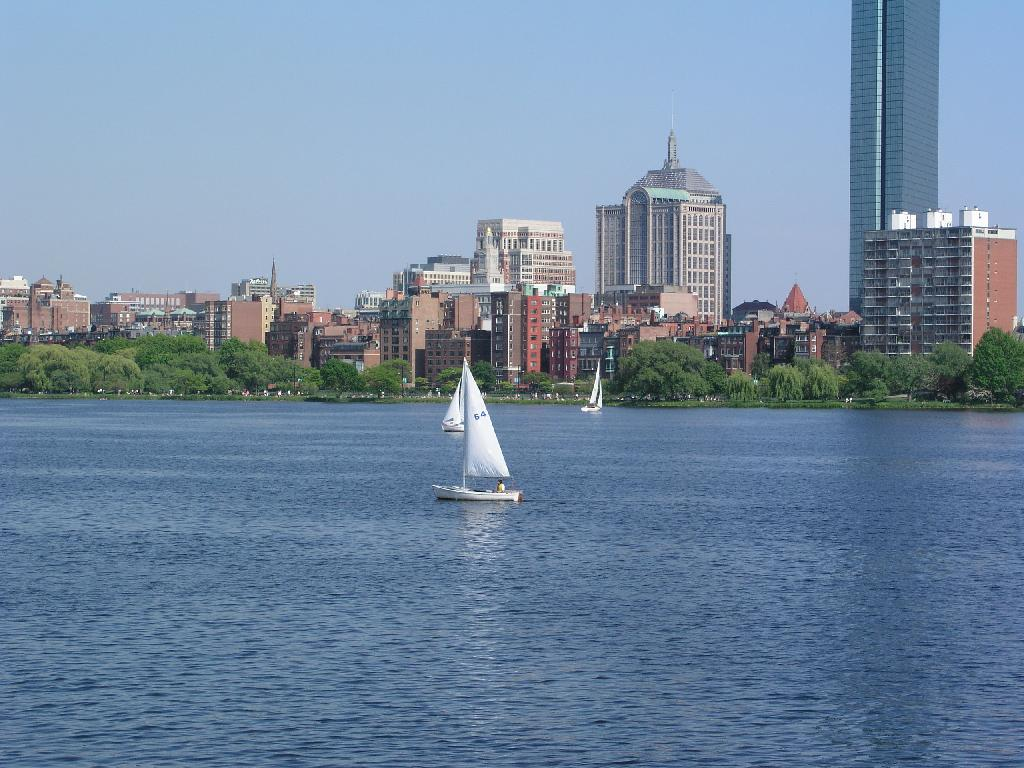
\includegraphics[width=0.9\linewidth]{visualInformation.jpeg}
  \newline
  \usebox{\mysaveboxTwo}
  \end{center}}
  
   \only<3>{
  \begin{center}
  \begin{align}
  1024 \times 768 \times 3 \times 8 = 18874368 bit\nonumber
  \end{align}
  \newline
  \usebox{\mysaveboxThree}
  \end{center}}
  
  \only<4>{
  \begin{center}
  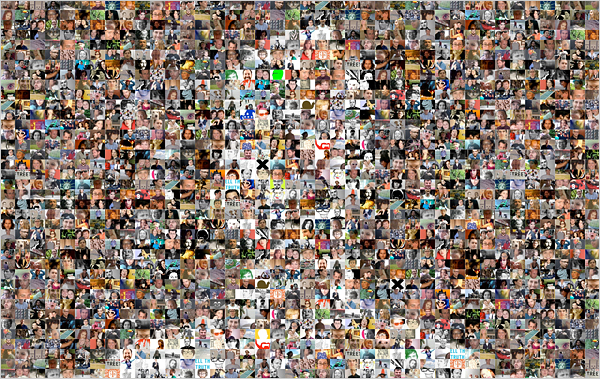
\includegraphics[width=1\linewidth]{people}
  \newline
  \usebox{\mysaveboxFour}
  \end{center}}
\end{frame}


\begin{frame}
\frametitle{What?}
\begin{figure}[!ht]
  \begin{minipage}[t]{0.46\textwidth}
  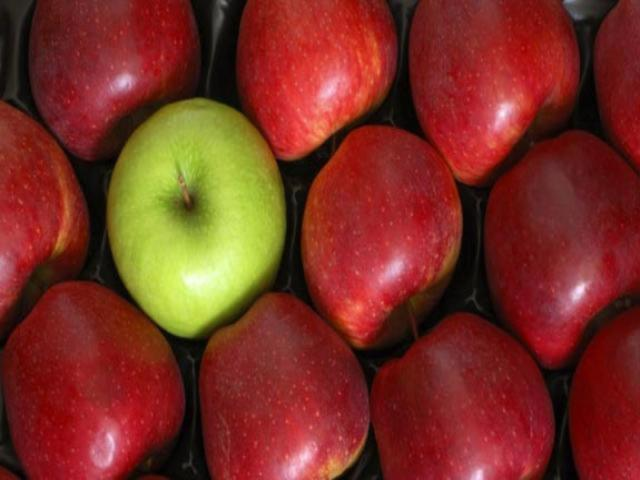
\includegraphics[width=1.8in]{apple1}
  \caption{Bottom-Up}
  \end{minipage}
  \begin{minipage}[t]{0.46\textwidth}
  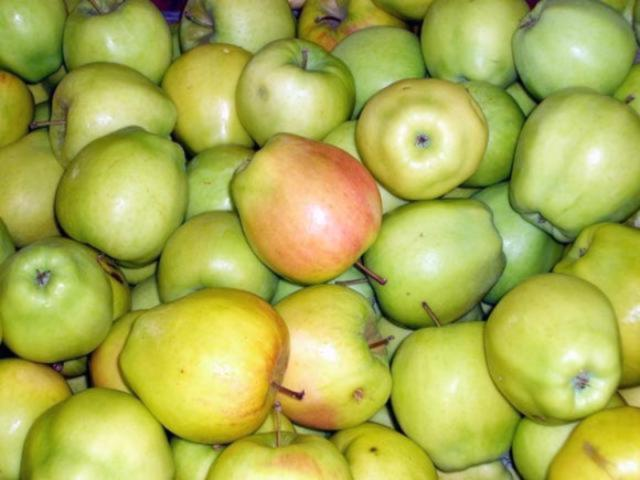
\includegraphics[width=1.8in]{apple2}
  \caption{Top-Down}
  \end{minipage}
  \end{figure} 
\end{frame}


\begin{frame}
\frametitle{Visual Attention}
\centering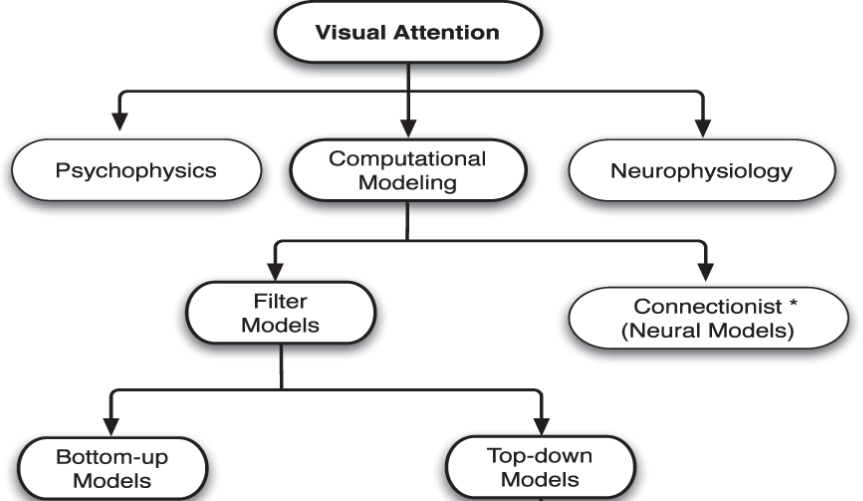
\includegraphics[width=10cm]{VisualAttention}
\end{frame}


\begin{frame}
\frametitle{Origins}
\begin{itemize}
\item ``Feature Integration Theory'', Treisman \& Gelade, 1980.
\item ``Guided Search Theory'', Wolfe \& Cave, 1989.
\item ``Integrated Competition Theory'', Desimone \& Duncan, 1995.
\end{itemize}
\end{frame}


\begin{frame}
\frametitle{Origins}
Koch and Ulman\footnote{C. Koch and S. Ullman, ``Shifts in selective visual attention: towards the underlying neural circuitry'', Human Neurobiology, 1985.} proposed a feed-forward model to combine features and introduced the concept of a saliency map which is a topographic map that represents conspicuousness of scene locations.
\end{frame}


\begin{frame}
\frametitle{Basic Structure of Computational Models}
\centering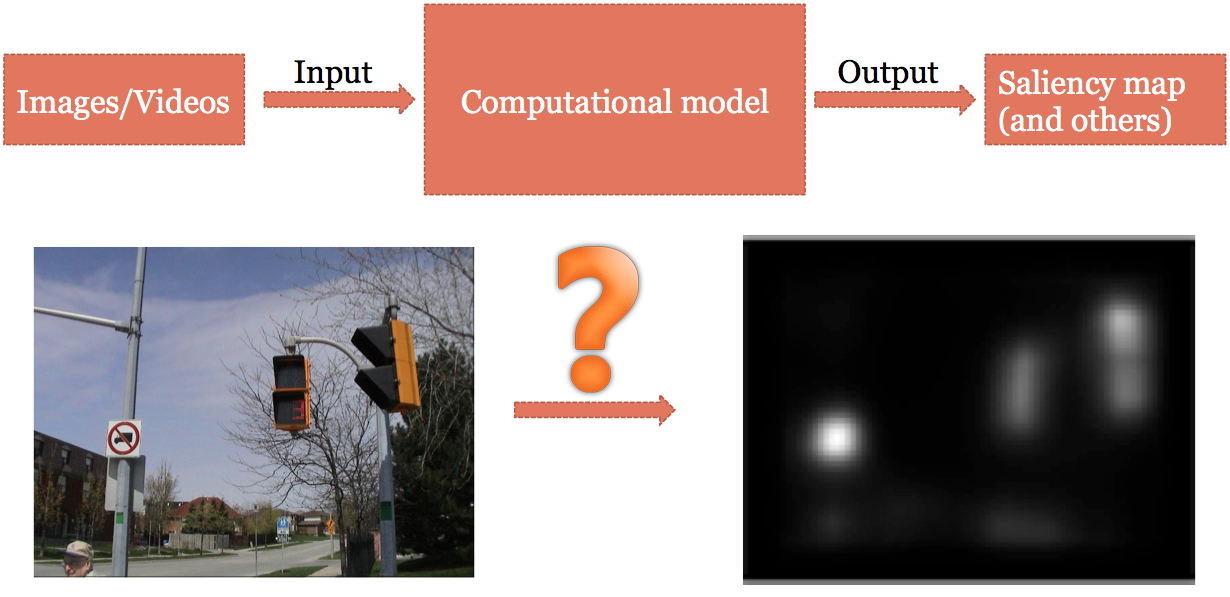
\includegraphics[width=10cm]{BasicStructure.jpg}
\end{frame}


\begin{frame}
\frametitle{Two Waves}
\centering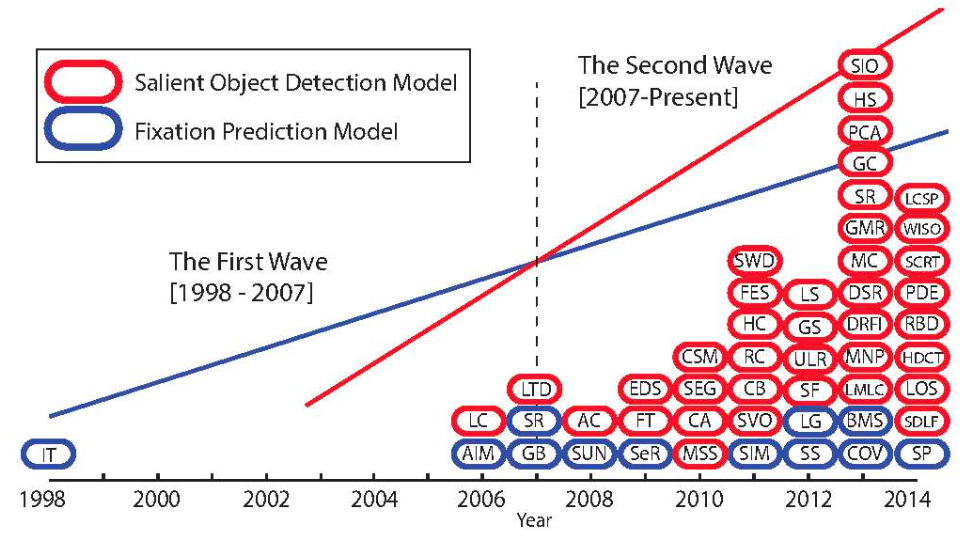
\includegraphics[width=10cm]{wave}
\end{frame}


\begin{frame}
\frametitle{Fixation Prediction}
Fixation prediction models are constructed originally to understand human visual attention and eye movement prediction.

\centering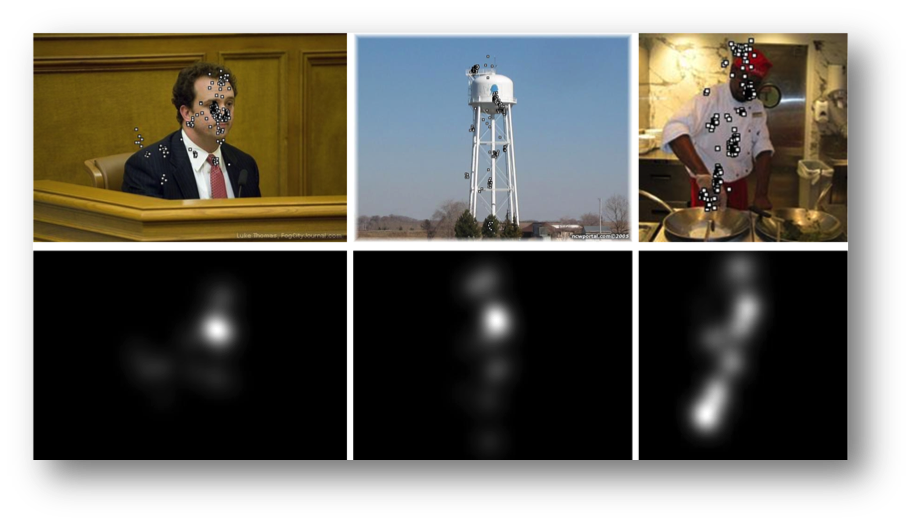
\includegraphics[width=8cm]{fixationPrediction.png}
\end{frame}

\begin{frame}
\frametitle{Representative Method}
\begin{itemize}
\item A model of saliency-based visual attention for rapid scene analysis. PAMI 1998, Itti et al.
\end{itemize}
\begin{figure}[!ht]
  \begin{minipage}[t]{0.45\textwidth}
  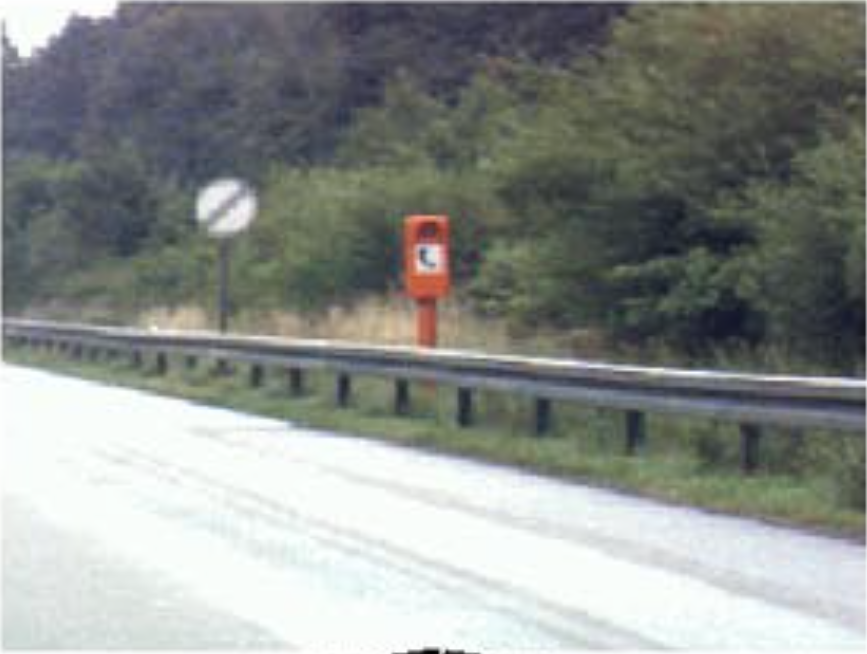
\includegraphics[width=1.8in]{sign}
  \end{minipage}
  \begin{minipage}[t]{0.45\textwidth}
  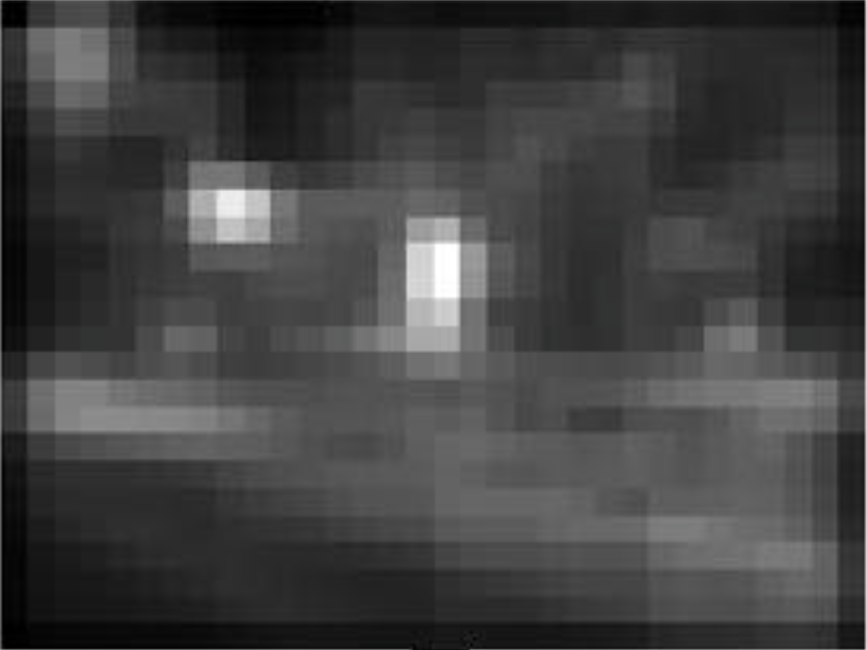
\includegraphics[width=1.8in]{signSaliency}
  \end{minipage}
  \end{figure} 
\end{frame}


\begin{frame}
\frametitle{Architecture}
\begin{figure}
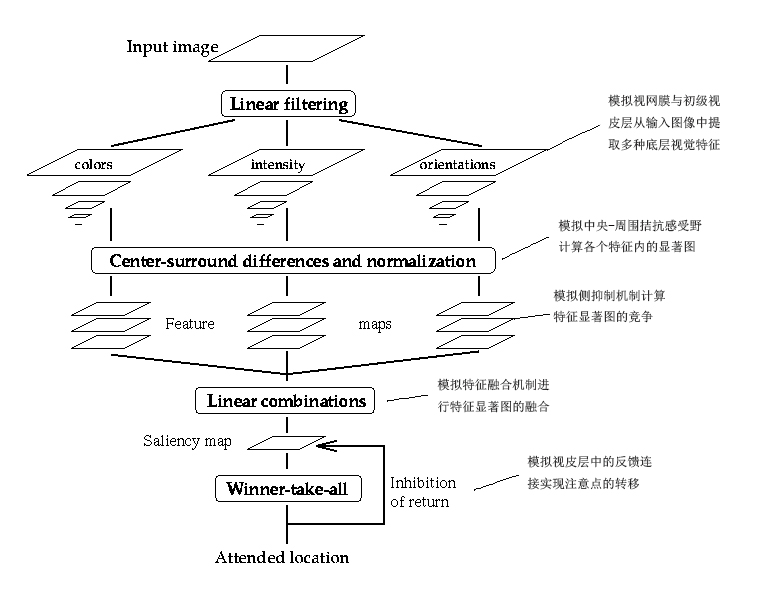
\includegraphics[width=10cm]{ITTImodel.png}
\end{figure}
\end{frame}


\begin{frame}
\frametitle{General Procedure of fixation prediction models}
\centering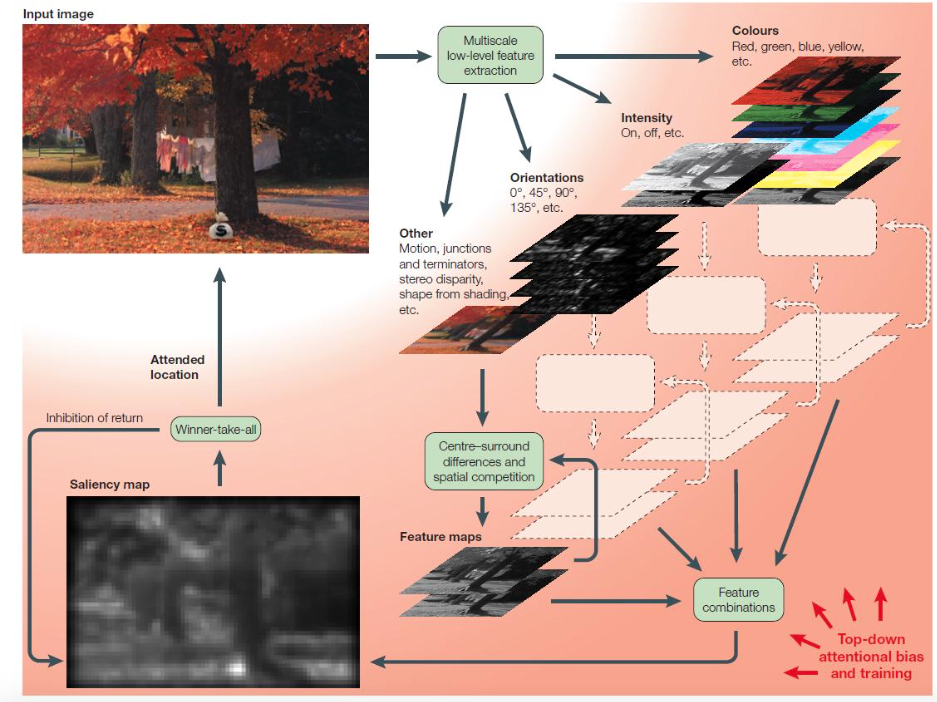
\includegraphics[width=10cm]{fixationArchitecture}
\end{frame}


\begin{frame}
\frametitle{How to evaluate fixation prediction models?}
\centering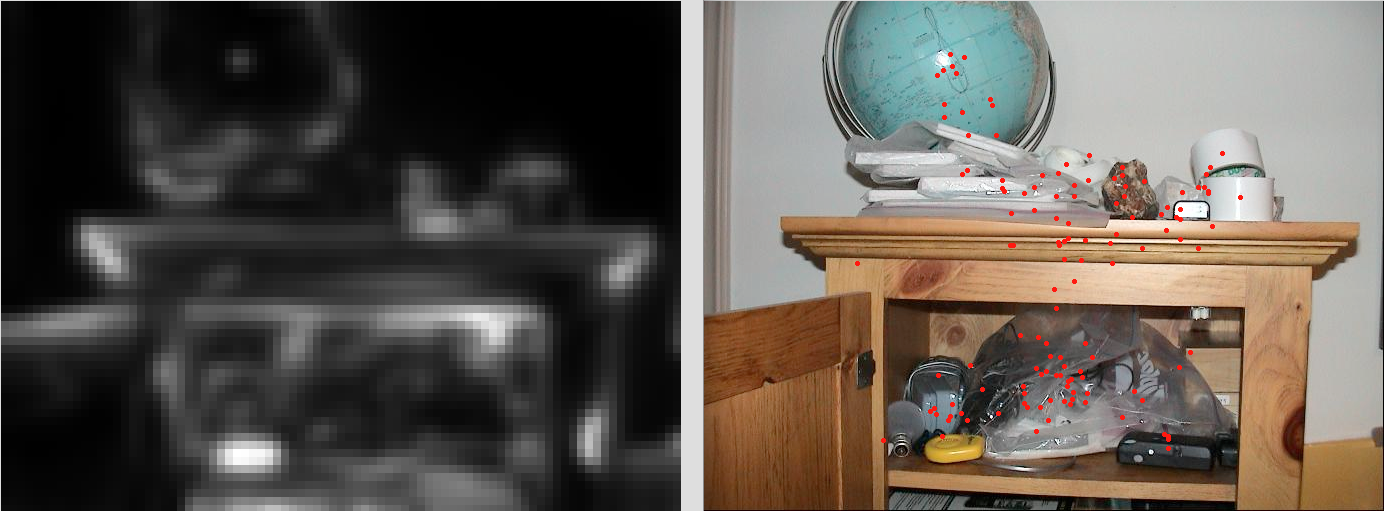
\includegraphics[width=10cm]{evaluateFixationModel}
\end{frame}


\begin{frame}
\frametitle{Salient Object Detection}
\centering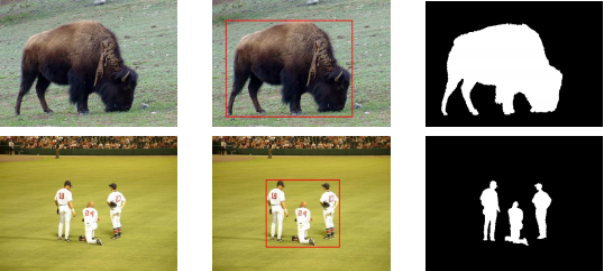
\includegraphics[width=7cm]{FT.png}
\begin{itemize}
\item Learning to detect a salient object. CVPR 2007, Tie Liu et al.
\item Frequency-tuned salient region detection. CVPR 2009, Achanta et al.
\end{itemize}
\end{frame}


\begin{frame}
\frametitle{Salient Object Detection}
\begin{itemize}
\item {\color{blue}\emph{Block-based}} vs. {\color{blue}\emph{Region-based analysis}}

Blocks are usually adopted by many early approaches, while regions are increasingly popular with the development of superpixel algorithms.

\item {\color{blue}\emph{Intrinsic cues}} vs. {\color{blue}\emph{Extrinsic cues}}
\end{itemize}
\end{frame}


\begin{frame}
\frametitle{Salient Object Detection}
Salient object detection is widely defined as capturing the uniqueness, distinctiveness, or rarity of a scene.

\begin{textblock*}{10cm}(2cm,2cm)
\rowcolors[]{1}{blue!20}{blue!10}
\begin{tabular}{ccc}
\multicolumn{3}{c}{Uniqueness}\\
Local Contrast & Global Contrast & Multi-scale Contrast 
\end{tabular}
\end{textblock*}

\begin{itemize}
\item Pixel-based 
\item Region-based
\end{itemize}
\end{frame}


\begin{frame}
\frametitle{Why? }
The emergence of salient object detection models is driven by the requirement of saliency-based applications.
\begin{figure}[!ht]
  \begin{minipage}[t]{0.4\textwidth}
  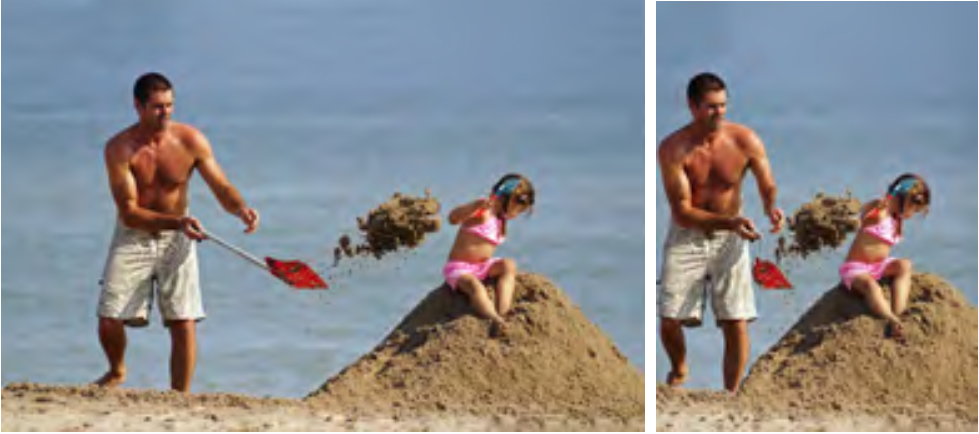
\includegraphics[height=0.7in]{resizing}
  \caption{Content aware resizing}
  \end{minipage}
  \begin{minipage}[t]{0.4\textwidth}
  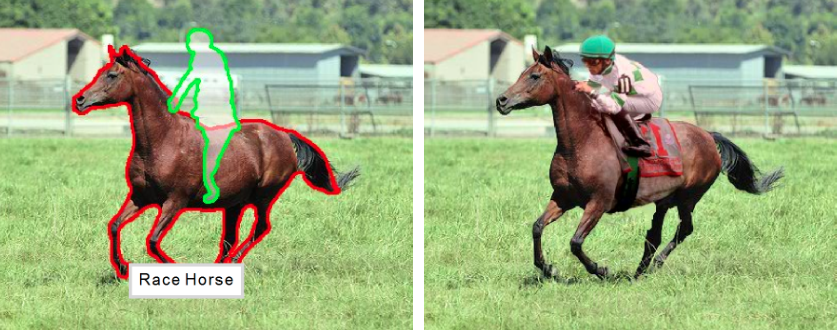
\includegraphics[height=0.7in]{manipulation}
  \caption{Object maniputation}
  \end{minipage}

\hspace{0.28in}
  \begin{minipage}[t]{0.4\textwidth}
  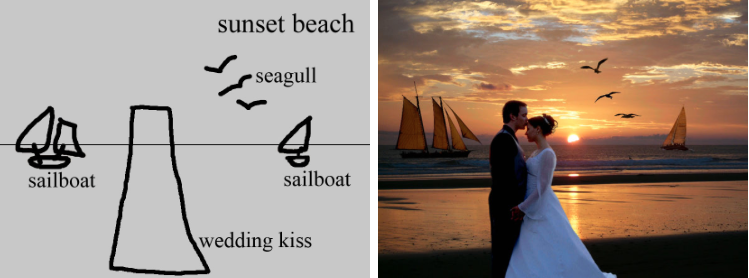
\includegraphics[height=0.7in]{sketch2photo}
  \caption{Image montage}
  \end{minipage}
  \begin{minipage}[t]{0.4\textwidth}
  \hspace{0.35in}
  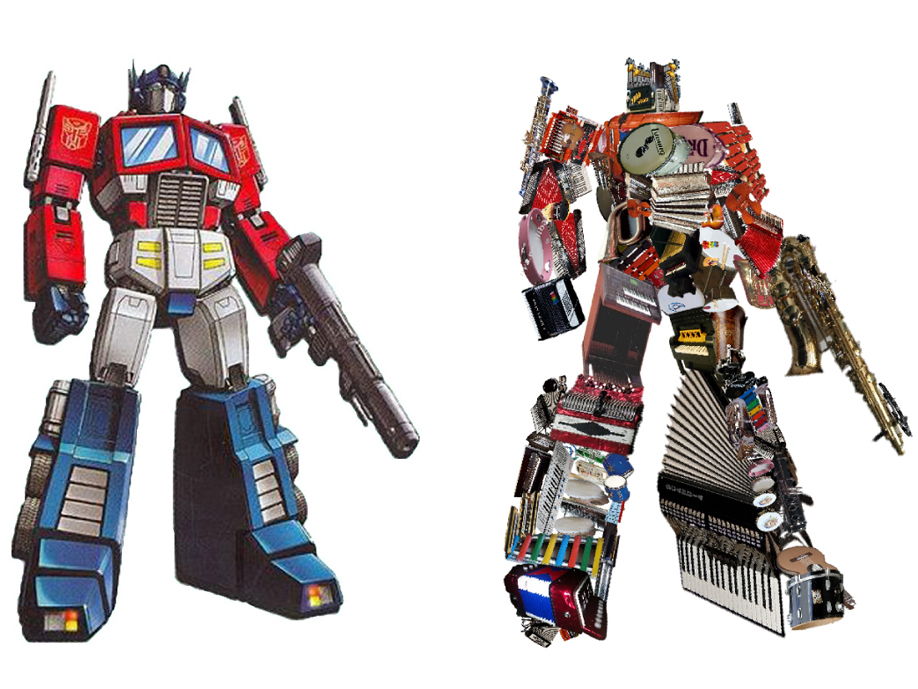
\includegraphics[height=0.7in]{collage.jpg}
  \caption{Image collage}
  \end{minipage}
\end{figure} 
\end{frame}


\begin{frame}
\frametitle{What can saliency not do?}
\centering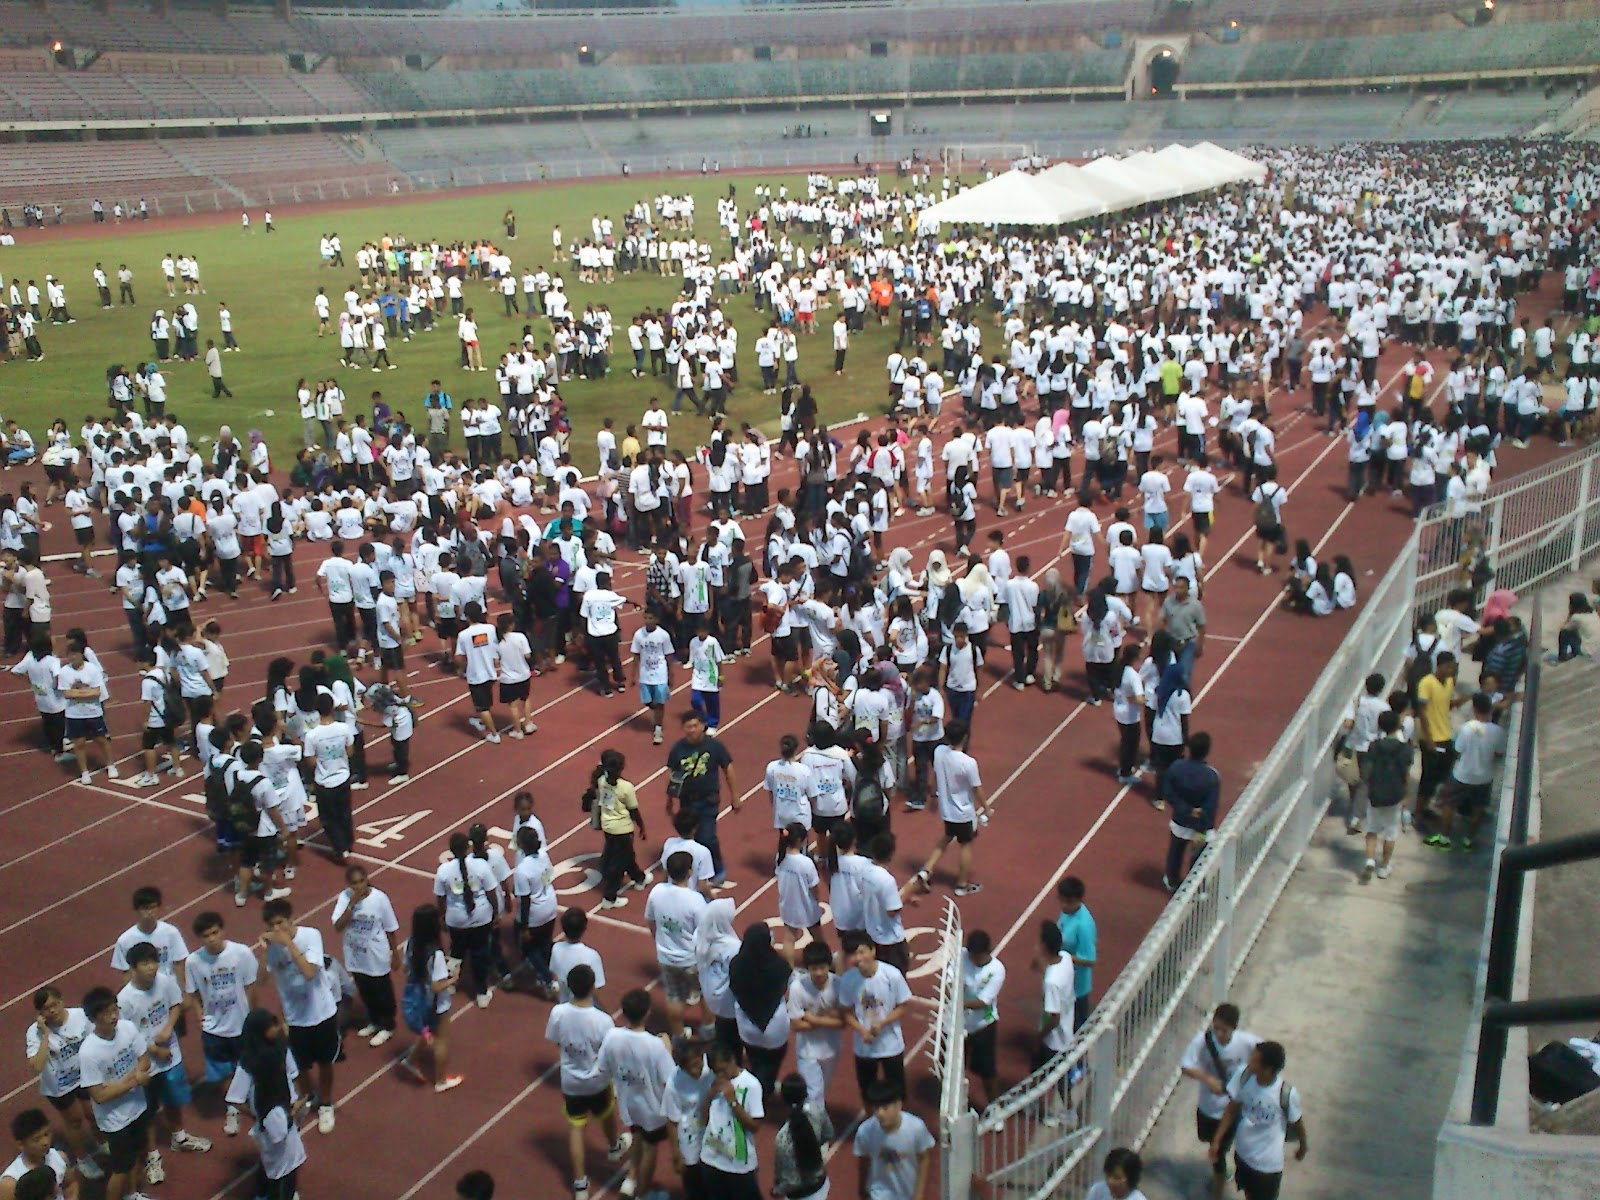
\includegraphics[width=9cm]{challenge.JPG}
\end{frame}


\begin{frame}
\frametitle{Latest research achievements}
\centering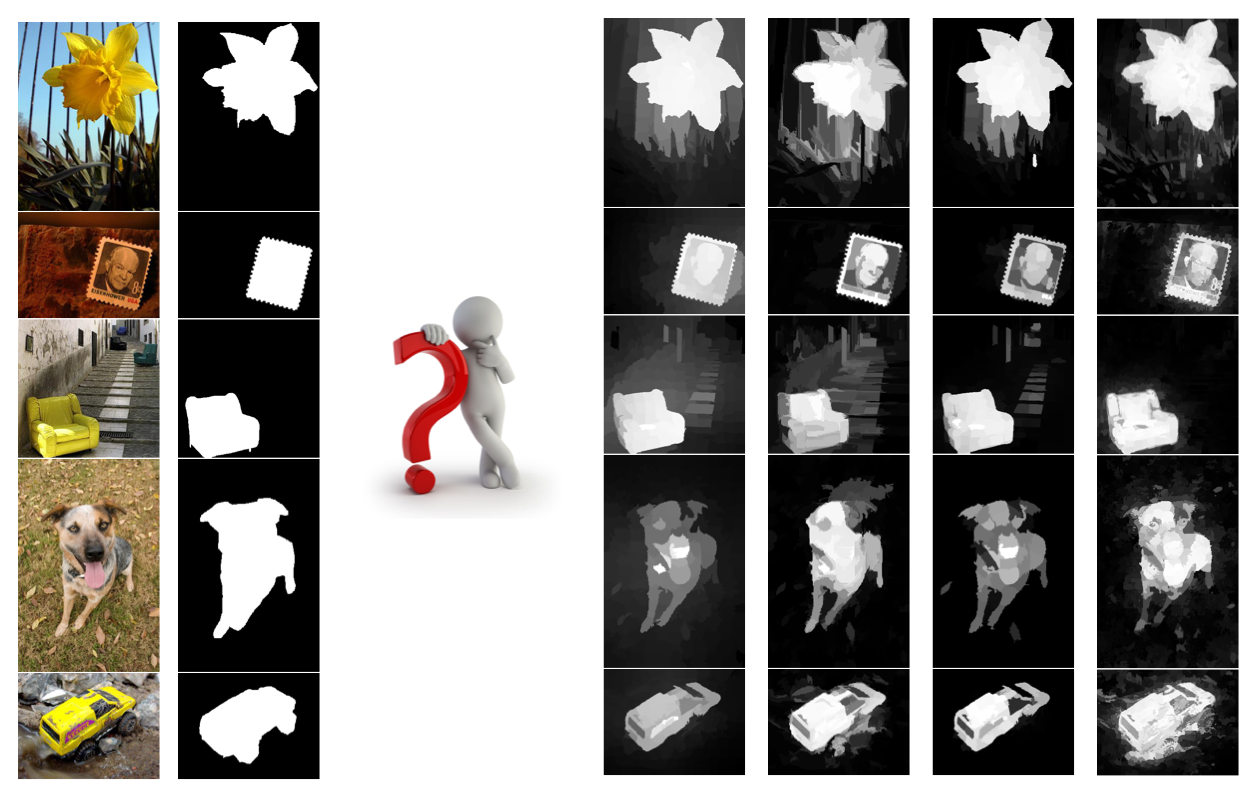
\includegraphics[width=6cm]{latest}

  From left to right: PBS\footnote{Chuan Yang et al, ``Graph-regularized saliency detection with convex-hull-based center prior, IEEE Signal Processing Letters, 2013.}、DRFI\footnote{Huaizu Jiang et al, ``Salient object detection: a discriminative regional feature integration approach'', in CVPR, 2013.}、RBD\footnote{Wangjiang Zhu et al, ``Saliency optimization from robust background detection'', in CVPR, 2014.}、HDCT\footnote{Jiwhan Kim et al, ``Salient region detection via high-dimensional color transform'', in CVPR, 2014.}
\end{frame}


\section{Features}

\begin{frame}
\frametitle{What are features?}
An image feature is a general term but it usually means a part of an image that contains interesting details or a property of the image which we are interested in.
\begin{columns}
\begin{column}{\leftmargini}
\end{column}
\begin{column}{0.5\linewidth}
\centering
\includegraphics[width=4cm]{image}
\end{column}
\begin{column}{0.7\linewidth}
\begin{itemize}
\item Edges
\item Points
\item Regions
\end{itemize}
\end{column}
\end{columns}\vspace{1ex}
\end{frame}


\begin{frame}
\frametitle{Features}
\begin{itemize}
\item Color feature
\item Texture feature
\item Geometric features
\end{itemize}
\end{frame}


\begin{frame}
\frametitle{Color}
\begin{itemize}
\item {\color{blue}\emph{Color}} is the visual perceptual property corresponding in humans to the categories called red, blue, yellow and others.
\item {\color{blue}\emph{Color Space}} is defined to identify colors numerically by their coordinates.
\end{itemize}
\end{frame}


\begin{frame}
\frametitle{Three Elements of Color}
\begin{itemize}
\item Hue: What we think as ``color''--yellow, orange, cyan and magenta are examples of different hues
\item Saturation: Saturation refers to the relative purity or the amount of white light mixed with a hue
\item Intensity
\end{itemize}
\centering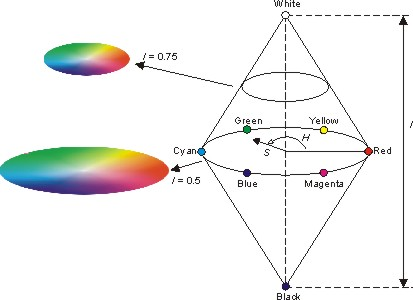
\includegraphics[width=6cm]{HSIColorModel.jpg}
\end{frame}


\begin{frame}
\frametitle{Coding methods for humans}
\begin{itemize}
\item \textbf{RGB} is an additive system (add colors to black) used for displays.
\item \textbf{CMY} is a subtractive system for printing.
\item \textbf{HSI} is a good perceptual space for art, psychology, and recognition.
\item \textbf{YIQ} is used for TV and is good for compression. 
\end{itemize}
\end{frame}


\begin{frame}
\frametitle{Device-dependent spaces}
\begin{itemize}
\item RGB、CMYK
\end{itemize}

\centering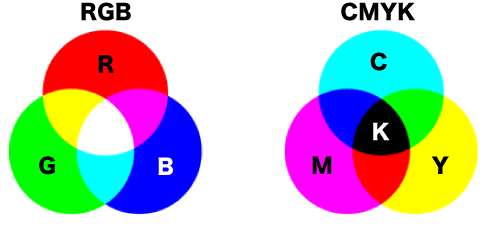
\includegraphics[width=7cm]{RGB_CMYK.png}
\end{frame}


\begin{frame}
\frametitle{Transformation}
Almost all the color spaces can be transformed from RGB color space.

\centering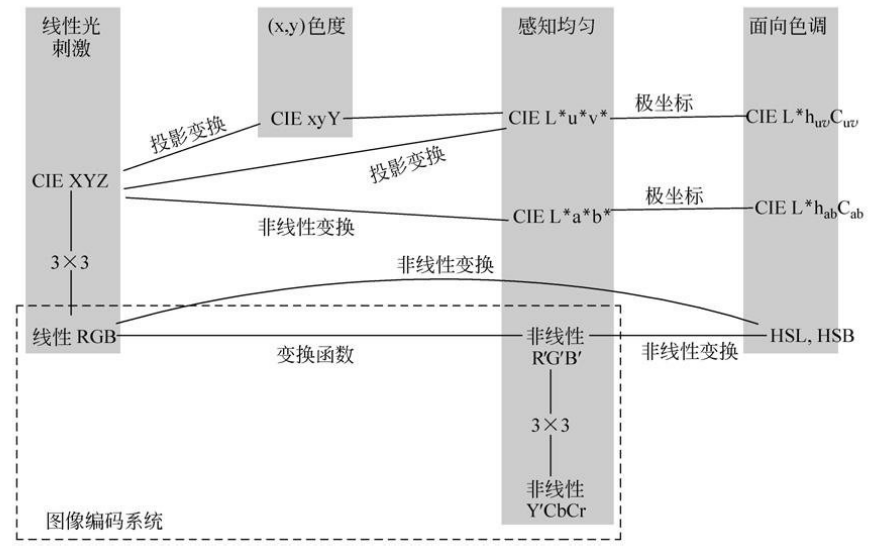
\includegraphics[width=8cm]{ColorSpaceTransform}
\end{frame}


\begin{frame}
\frametitle{Edges}
Edges are points that are at the boundary of two image regions and are detected by computing the change in brightness.

\centering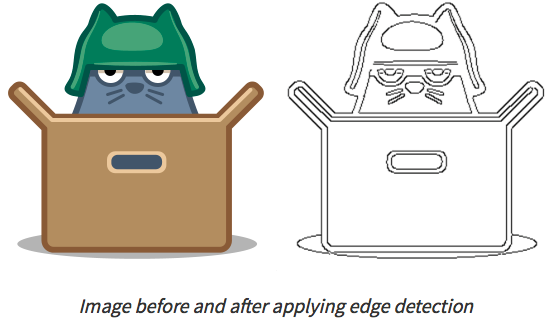
\includegraphics[width=8cm]{edge}
\end{frame}


\begin{frame}
\frametitle{Corners/interest points}
A corner is the point located at the intersection of two edges and you can think of an interest point as a small region in the image(window) for which no matter in which neighboring direction you look there is a high variations in brightness.

\centering
\includegraphics[width=5cm]{corner}
\end{frame}


\begin{frame}
\frametitle{Blobs/regions of interest}
Blobs, or regions of interest, are regions where the brightness or color of the points change very little so they can be considered in some sense to be similar to each other.

\centering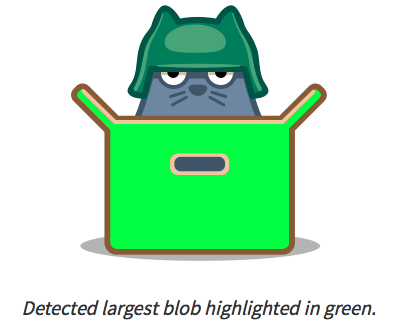
\includegraphics[width=6cm]{blob}
\end{frame}


\begin{frame}
\frametitle{\emph{feature} vs \emph{feature descriptor}}
\begin{description}
\item[Feature detection] A low-level image processing operation and it examines every pixel to see if the region around that pixel could be used as a feature.
\item[Feature description] Once the features that are interesting to us have been detected, they can be extracted. The result is known as a feature descriptor or feature vector and they characterize the region around the key point.
\end{description}
\end{frame}


\begin{frame}
\frametitle{Feature Descriptor}
\begin{itemize}
\item Invariance
\item Distinguishability
\end{itemize}
SIFT、、
\end{frame}


\begin{frame}
\frametitle{Steps}
\centering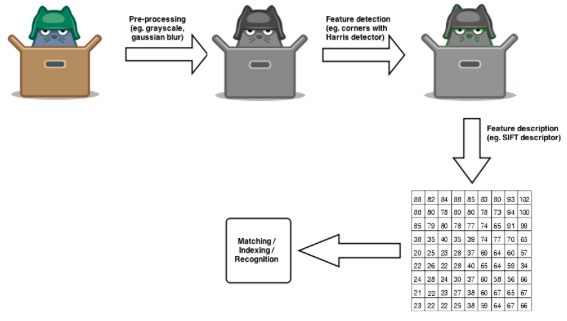
\includegraphics[width=10cm]{steps}
\end{frame}


\begin{frame}
\frametitle{What is texture?}
Texture is actually a very nebulous concept, often attributed to human perception, as either the feel or the appearance of (woven) fabric.\footnote{Mark S.Nixon and Alberto S.Aguado, ``Feature Extraction \& Image Processing for Computer Vision'', Publishing House of Electronics Industry, 2013.}
\end{frame}


\begin{frame}
\frametitle{Texture Descriptor}
\begin{itemize}
\item Structural approaches
\item Statistical approaches
\item Combination approaches
\item Local binary patterns
\end{itemize}
\end{frame}


\begin{frame}
\frametitle{LBP(Local Binary Pattern,局部二值模式)}
\centering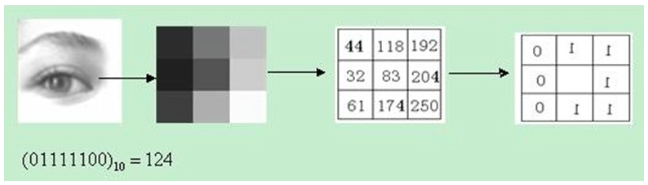
\includegraphics[width=10cm]{LBP.png}
\end{frame}


\begin{frame}
\frametitle{LBP}
  \begin{figure}[!ht]
  \begin{minipage}[t]{0.46\textwidth}
  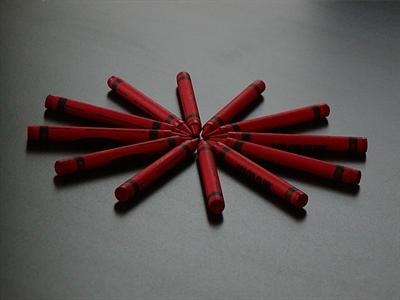
\includegraphics[width=1.8in]{example1.jpg}
  \end{minipage}
  \begin{minipage}[t]{0.46\textwidth}
  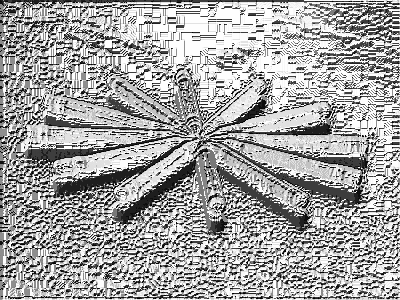
\includegraphics[width=1.8in]{LBP1.png}
  \end{minipage}
  \end{figure} 
\end{frame}


\begin{frame}
\frametitle{Regional property descriptor}
\begin{itemize}
\item Appearance feature descriptor
\item Geometric feature descriptor
\end{itemize}
\end{frame}


\begin{frame}
\frametitle{Regional contrast descriptor}

\end{frame}


\section{Priors}

\begin{frame}
\frametitle{Priors}
\begin{itemize}
\item Center Prior/Location Prior
\item Backgroundness Prior
\item Boundary Connectivity Prior
\item Color Prior
\item Objectness Prior
\item Smoothness Prior
\end{itemize}
\end{frame}


\begin{frame}
\frametitle{Center Prior/Location Prior}
{\color{blue}Objects near the image center are more attractive to people.}\footnote{Zhang, Lin and Gu, Zhongyi and Li, Hongyu, ``SDSP: A novel saliency detection method by combining simple priors'', in ICIP, 2013.}

\vspace{0.15in}

This prior can be simply and effectively modeled as a Gaussian map.

\vspace{0.15in}

\begin{columns}
\begin{column}{\leftmargini}
\end{column}
\hspace{-1in}
\begin{column}{0.1\linewidth}
\centering
\includegraphics[width=3cm]{CenterPrior}
\end{column}
\begin{column}{0.7\linewidth}
\begin{align}
S_D(\textbf{x}) = exp\left(-\frac{||\textbf{x}-\textbf{c}||_2^2}{\sigma_D^2}\right)
\end{align}
\end{column}
\end{columns}\vspace{1ex}
\vspace{-0.4in}
\end{frame}


\begin{frame}
\frametitle{Center Prior/Location Prior}
{\color{blue}The salient object in an image is most probably placed near the center of the image.}\footnote{Jiang, Huaizu and Wang, Jingdong, "Automatic salient object segmentation based on context and shape prior", in BMVC, 2011}

\vspace{0.2in}

Gaussian falloff weight:
\begin{align}
w_i^{(n)} = exp(-9(dx_i^{(n)})^2/w^2-9(dy_i^{(n)})^2/h^2
\end{align}

\centering
\includegraphics[width=3cm]{CBcolorPrior.png}
\end{frame}


\begin{frame}
\frametitle{Center Prior/Location Prior}
Assigning higher saliency to the image elements near the image center becomes invalid when the objects are placed far off the image center\footnote{Yang, Chuan and Zhang, Lihe and Lu, Huchuan, ``Graph-regularized saliency detection with convex-hull-based center prior'', in Signal Processing Letters, IEEE, 2013}.
\begin{columns}
\begin{column}{\leftmargini}
\end{column}
\begin{column}{0.5\linewidth}
\begin{itemize}
\item Compute a convex hull enclosing interesting points to estimate the location of salient region.
\item Use the centroid of the convex hull as the center to get the convex-hull-based center prior map.
\end{itemize}
\end{column}
\begin{column}{0.5\linewidth}
\centering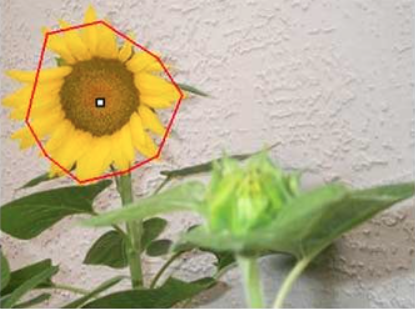
\includegraphics[width=4cm]{convexHull}
\end{column}
\end{columns}\vspace{1ex}
\end{frame}


\begin{frame}
\frametitle{Backgroundness Prior}
{\color{blue}\emph{Backgroundness prior}} is more general than center prior because salient objects can be placed off the center, but they seldom touch the image boundary.\footnote{Wei, Yichen and Wen, Fang and Zhu, Wangjiang, ``Geodesic saliency using background priors'', in ECCV, 2012.}
\begin{itemize}
\item Assuming that a narrow border of the image is background region, regional saliency can be computer as the contrast versus ``background''.
\end{itemize}
\vspace{0.3in}
\end{frame}


\begin{frame}
\frametitle{Boundary Connectivity Prior}
{\color{blue}Object regions are much less connected to image boundaries than background ones.}\footnote{Zhu, Wangjiang and Liang, Shuang, ``Saliency optimization from robust background detection'', in CVPR, 2014.}

\centering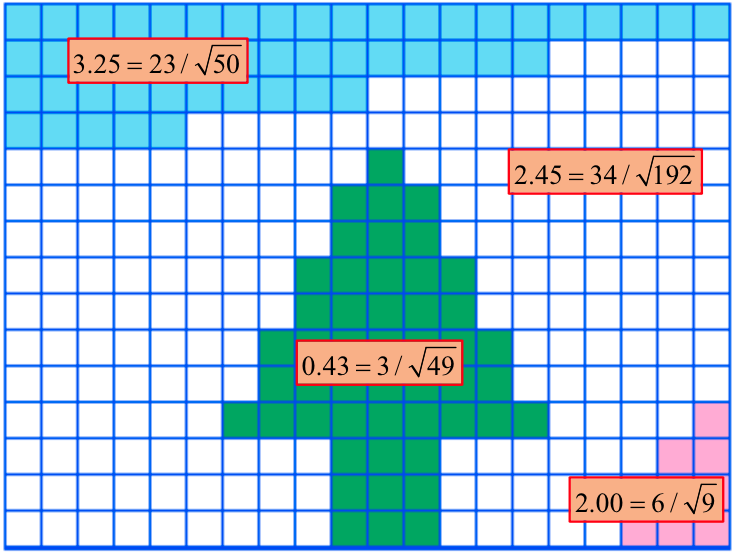
\includegraphics[width=4cm]{wCtr.png}

\emph{Boundary connectivity} is defined to quantify how heavily a region R is connected to the image boundaries.
\begin{align}
BndCon(R) = \frac{|\{p|p\in R, p\in Bnd\}|}{\sqrt{|\{p|p\in R\}|}}
\end{align}
\end{frame}


\begin{frame}
\frametitle{Color Prior}
{\color{blue}Warm colors, such as red and yellow, are more pronounced to the human visual system than cold colors, such as green and blue.}\footnote{Zhang, Lin and Gu, Zhongyi and Li, Hongyu, ``SDSP: A novel saliency detection method by combining simple priors'', in ICIP, 2013.}
\begin{align}
f_{an}(\textbf{x}) & =\frac{f_a(x)-mina}{maxa-mina}, f_{bn}(\textbf{x}) = \frac{f_b(x)-minb}{maxb-minb}\\
S_c(\textbf{x}) & = 1-exp\left(-\frac{f_{an}^2(\textbf{x})+f_{bn}^2(\textbf{x})}{\sigma_c^2}\right)
\end{align}
\begin{itemize}
\item $a^*$-channel represents green-red information
\item $b^*$-channel represents blue-yellow information
\end{itemize}
\end{frame}


\begin{frame}
\frametitle{Objectness Prior}
{\color{blue}\emph{Objectness}} is defined as the probability of there being a complete object in a local window centered on each pixel.\footnote{Jiang, Peng and Ling, Haibin, ``Salient region detection by ufo: uniqueness, focusness and objectness'', in ICCV, 2013} 
\begin{itemize}
\item Randomly sample $N$ windows over the image 
\item Assign each window $w$ a probability score $P(w)$ to indicate its objectless
\item Sum all the probability scores in windows that contains pixel $x$
\end{itemize}
\begin{align}
O_p(x) = \sum_{w \in W \text{ }and \text{ } x \in w} P(W_x)
\end{align}
\end{frame}


\begin{frame}
\frametitle{Smoothness Prior}
{\color{blue}\emph{Smoothness}} constraint is often encoded by adding a pair-wise potential to the energy function which encourages neighboring pixels in the image to take the same label.\footnote{Yang, Chuan and Zhang, Lihe and Lu, Huchuan, ``Graph-regularized saliency detection with convex-hull-based center prior'', in Signal Processing Letters, IEEE, 2013.}
\begin{align}
w_{ij} & = exp\left(-\frac{||c_i-c_j||}{2\sigma_w^2}\right)\\
E(S) & = \sum_{i}(S(i)-S_in(i))^2+\lambda \sum_{i, j}w_{ij}(S(i)-S(j))^2
\end{align}
\end{frame}


\begin{frame}
\frametitle{SDSP\footnote{Zhang, Lin and Gu, Zhongyi and Li, Hongyu, ``SDSP: A novel saliency detection method by combining simple priors'', in ICIP, 2013.}}

\centering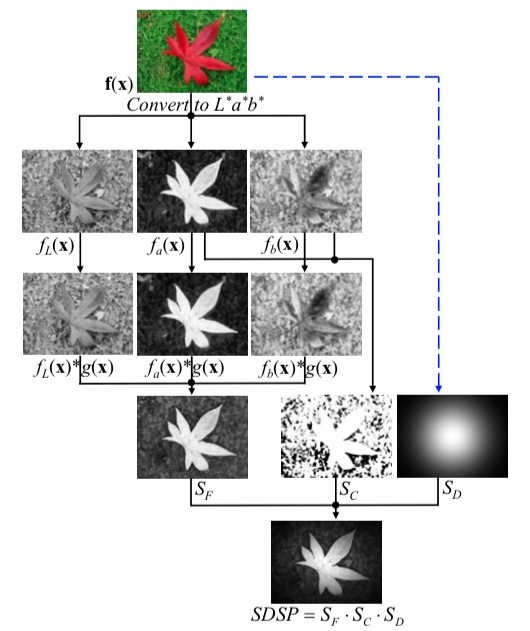
\includegraphics[width=5.7cm]{SDSP}
\end{frame}


\section{Integration}

\begin{frame}
\frametitle{Optimization\footnote{Wangjiang Zhu and Shuang Liang, ``Saliency Optimization from Robust Background Detection, in CVPR, 2014.}}
The ideal output of salient object detection is a clean binary object/background segmentation.

\centering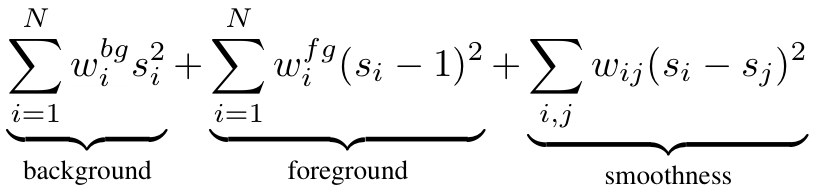
\includegraphics[width=6cm]{optimization}
\end{frame}



\begin{frame}
  \vspace{2cm}
  \centering
  \zhushadow{\color{blue}\Huge{Thanks}}\\
  \vspace{1.5cm}
  \begin{flushright}
  \emph{\href{zhuyafei4520@163.com}{Yafei~Zhu}}\\
  \href{http://www.ouc.edu.cn}{Ocean University of China}\\
  \emph{2015.03}
  \end{flushright}  
\end{frame}

%===============================================================================


\end{document}
